% Created 2021-04-20 Tue 20:37
% Intended LaTeX compiler: pdflatex
\documentclass[12pt,paper=a4,oneside,hidelinks,headings=small,captions=heading,captions=nooneline]{scrartcl}
                \usepackage{microtype}
                \usepackage{tgpagella}
                \usepackage[scale=.9]{tgheros}
                \usepackage{tgcursor}
                \usepackage{paralist}
                \newcommand{\rc}{$^{14}C$}
\usepackage[utf8]{inputenc}
\usepackage[T1]{fontenc}
\usepackage{graphicx}
\usepackage{grffile}
\usepackage{longtable}
\usepackage{wrapfig}
\usepackage{rotating}
\usepackage[normalem]{ulem}
\usepackage{amsmath}
\usepackage{textcomp}
\usepackage{amssymb}
\usepackage{capt-of}
\usepackage{hyperref}
\usepackage[T1]{fontenc} %\hypersetup{colorlinks=true}
\usepackage{titlesec} \usepackage{lipsum}\usepackage{indentfirst}\setlength{\parindent}{3em}
\usepackage[tmargin=2.5cm, bmargin=2cm,inner=2.5cm,outer=2.5cm]{geometry}
\usepackage[sfdefault]{libertine} % sans = Linux Biolinum
\usepackage{fancyhdr}\pagestyle{fancyplain}\fancyhf{}
\renewcommand{\plainheadrulewidth}{0pt}\fancyhead[R]{\thepage}
\renewcommand{\headrulewidth}{0pt}
\renewcommand*\oldstylenums[1]{{\fontfamily{fxlj}\selectfont #1}}
\usepackage{lmodern}
\titleformat{\section}{\normalfont\centering\bfseries}{\thesection}{1em}{}
\titleformat{\subsection}{\normalfont\bfseries}{\thesubsection}{1em}{}
\titleformat{\subsubsection}{\normalfont\bfseries\itshape}{\thesubsubsection}{1em}{}
\titleformat{\paragraph}[runin]{\normalfont\bfseries}{\theparagraph.}{1em}{}[.]\titlespacing{\paragraph}{\parindent}{0pt}{4pt}
\titleformat{\subparagraph}[runin]{\normalfont\bfseries\itshape}{\thesubparagraph.}{1em}{}[. ]\titlespacing{\subparagraph}{\parindent}{0pt}{4pt}
\titleformat{\subsubparagraph}[runin]{\normalfont}{\thesubsubparagraph.}{1em}{}[. ]\titlespacing{\subsubparagraph}{\parindent}{0pt}{4pt}
\usepackage[hidelinks=true]{hyperref}
\usepackage[margin=1em,justification=centering]{caption}
\usepackage[ngerman, germanb]{babel}
\usepackage[utf8]{inputenc}
\usepackage[fixlanguage]{babelbib}\selectbiblanguage{austrian}
\usepackage{csquotes,xpatch}
\usepackage[natbib=true,style=apa,backend=biber,doi=true,url=true,eprint=false,hyperref=true,annotation=false]{biblatex}
\urlstyle{sf}
\DeclareLanguageMapping{austrian}{austrian-apa}
\DeclareSourcemap{\maps[datatype=bibtex]{\map{\step[fieldset=annotation,null]}}}
\addtolength\parskip{\medskipamount}
\usepackage{tabulary,booktabs,longtable}
\usepackage{caption}
\DeclareCaptionLabelSeparator{skipsep}{\vskip 1em} % APA 7 caption
\captionsetup[figure]{labelsep=skipsep}
\captionsetup[table]{labelsep=skipsep}
\addtokomafont{caption}{\itshape} % APA 7 italic figure/table captions
\setkomafont{captionlabel}{\normalfont\bfseries} % APA 7 bold figure/table caption labels
\renewcommand*{\captionformat}{\vskip 1.5em} % APA 7 caption
\setcaphanging
\setcapmargin*{0cm}
\setcapindent*{0pt}
\captionsetup{belowskip=1.5em,aboveskip=1.5em}% APA 7 distance between caption and figure/table
\BeforeBeginEnvironment{figure}{\vskip 1.5em}\AfterEndEnvironment{figure}{\vskip 1.5em}
\BeforeBeginEnvironment{table}{\vskip 1.5em}\AfterEndEnvironment{table}{\vskip 1.5em}
\AtBeginEnvironment{tabular}{\small}%
\author{Asım OĞUZ, Dominik PEGLER, Sophia PUM}
\date{\today}
\title{Meilenstein 2\\\medskip
\large HCI 2021S: Interior Designer}
\hypersetup{
 pdfauthor={Asım OĞUZ, Dominik PEGLER, Sophia PUM},
 pdftitle={Meilenstein 2},
 pdfkeywords={},
 pdfsubject={},
 pdfcreator={Emacs 27.2 (Org mode 9.4.4)}, 
 pdflang={Germanb}}
\begin{document}

\maketitle
\setcounter{tocdepth}{2}
\tableofcontents\newpage

\section{Ideensammlung}
\label{sec:orgfefda62}

\emph{Autor*innen: Dominik Pegler, Sophia Pum}

Um eine Vielfalt an Ideen möglichst umfangreich und vollständig
abbilden zu können und dabei nicht den Überblick zu verlieren, haben
wir uns für eine \textbf{Mind-Mapping-Technik} entschieden. Im ersten Schritt
haben wir uns gefragt, worum es sich bei unserem Projekt überhaupt
handelt. Die Antworten darauf bildeten sozusagen die erste Ebene
unserer Mindmap. In den Folgeschritten wurde diese erste Ebene
erweitert und um neue, darunterliegende, Ebenen ergänzt. Beim Grad der
Ausdifferenzierung der einzelnen Knotenpunkte haben wir uns kein Limit
gesetzt. Wir wollten erstmal nur sehen, welche Aspekte in uns mehr
Wunsch nach Detailreichtum auslösten.

Die weitere Strukturierung der Mindmap erfolgte zwei Tage
später. Die folgenden drei Aspekte möchten wir als für uns wichtig festhalten.

\begin{enumerate}
\item Es handelt sich um eine \textbf{mobile App}. Das bedeutet, dass wir den
Fokus besonders auf Simplizität der Bedienoberfläche und möglichst
verzögerungsfreie Rückmeldungen der Applikation an den User legen
werden. Mit Simplizität meinen wir konkret eine minimale Anzahl an
verschiedenartigen Screens, Text nur dort, wo es wirklich nötig ist
und es keine aussagekräftigen Icons gibt. Um die Aufmerksamkeit der
User nicht auf das Interface zu lenken, sondern davon weg auf deren
Aufgaben, vermeiden wir auch Hell-Dunkel- sowie Farbkontraste
überall dort, wo es nicht notwendig ist. Wir denken hier an
maximale Anzahl von 3 verschiedenen Farben. Die User sollen das
Gefühl haben, durch die App "`hindurchzublicken"'. Es soll ein
Werkzeug sein und nicht die ganze Aufmerksamkeit der User
erfordern.
\item Für das Design haben wir unterschiedliche Motivationen. Die
\textbf{Hauptfunktionen} aller Prototypen sollen das Einscannen,
Umgestalten und Einrichten von Räumen sein. In allen Entwürfen
möchten wir es ermöglichen, diese Funktion mit nur wenigen Klicks
einfach zu erreichen. Aussagekräftige Icons und Bilder sowie wenig
Text und eine reduzierte Anzahl von ScreensGenerell wollen wir
alle Prototypen klar und minimalisitsch designen, um eine
übersichtliche und simple Struktur zu bewahren. Bei der Gestaltung
der Nutzeroberfläche haben wir uns unter anderem von ähnlichen Apps
inspirieren lassen. Weiters soll es bei jedem Prototyp verschiedene
Lösungen geben, wie man gespeicherte Möbel durchschauen kann. Eine
Möglichkeit würde das über einen zusätzlichen Menüpunkt lösen, bei
dem man Möbel scannen, speichern und durchsuchen kann. In einer
weiteren Möglichkeit könnte es einen zweiten Punkt geben, in dem
man gespeicherte Räume ansehen und bearbeiten kann. Eine dritte
Möglichkeit wäre es noch, die Gestaltungsobjekte beim Raum selbst
designen zu können. All das möchten wir in Prototypen-Gestaltung
versuchen miteinzubeziehen.
\item Die Funktion des Scannens eigener Gegenstände möchten weiterhin im
Projekt behalten, da es für uns ein essenzieller Bestandteil des
Konzepts ist und unserer Meinung nach ein wichtiges \textbf{Argument für
die Verwendung} der App darstellt. Andere Anbieter erlauben es nur,
Gegenstände aus entweder dem eigenen Produktkatalog oder zumindest
aus einer limitierten Anzahl an Marken und Beispielmöbeln zum
Gestalten der Räume zu verwenden. Wir sehen diese Funktion nicht
nur als reine Funktion, sie ist auch nicht mal wesentlich für das
UI, aber als potenziell eigenständige Plattform zum Austausch von
Gegenständen, insbesondere von Möbelstücken. Auch wenn dies bereits
ein Projekt im Projekt darstellt, wollen wir wollen wir versuchen,
diese Funktionalität bei Designentscheidungen immer im Hinterkopf
zu behalten.

Aufgrund des Formats und der Größe ist unsere Mindmap nicht direkt
im Dokument angehängt, sie findet sich an \uline{\href{https://dominikpegler.github.io/interior-designer/img/mindmap.png}{dieser Stelle}}.
\end{enumerate}
\section{Low-Fi-Prototypen}
\label{sec:orge20236e}
\subsection{Prototyp von Sophia}
\label{sec:orgd451574}
\emph{Autorin: Sophia Pum}

Es gibt zwei Start-Screens (\textbf{Abb. \ref{fig:lofi_sophia_12}}), zwischen die man durch wischen navigieren
kann. Am ersten Screen sieht man den Schriftzug „Start Designing“ mit
einer kurzen Beschreibung darunter, was einem erwartet und einem
Button „Raum Designen“. Als Hintergrund würde ich ein schlichtes Bild
eines minimal gestalteten Raums einfügen. Danach erscheinen vier
Felder zum Auswählen, die jeweils mit einem Titel und einem Icon
gestaltet sind. Die ersten beiden Felder „Kamera“ und „Fotoalbum“
ermöglichen einen entweder direkt mit der Kamera oder mithilfe
gespeicherten Albumfotos den Raum einzuscannen und anschließend zu
bearbeiten. Ist der Raum fertig eingescannt kann man mithilfe des
Menü-Buttons rechts oben Möbel platzieren und andere Umgestaltungen
wie z.B. Wandfarbe ändern durchführen. Mit dem Feld „Leerer Raum“ kann
man einen komplett neuen Raum erstellen und gestalten und unter
„gespeicherte Räume“ findet man bereits bearbeitet Räum und kann diese
weiter anpassen.

\begin{figure}[htbp]
\centering
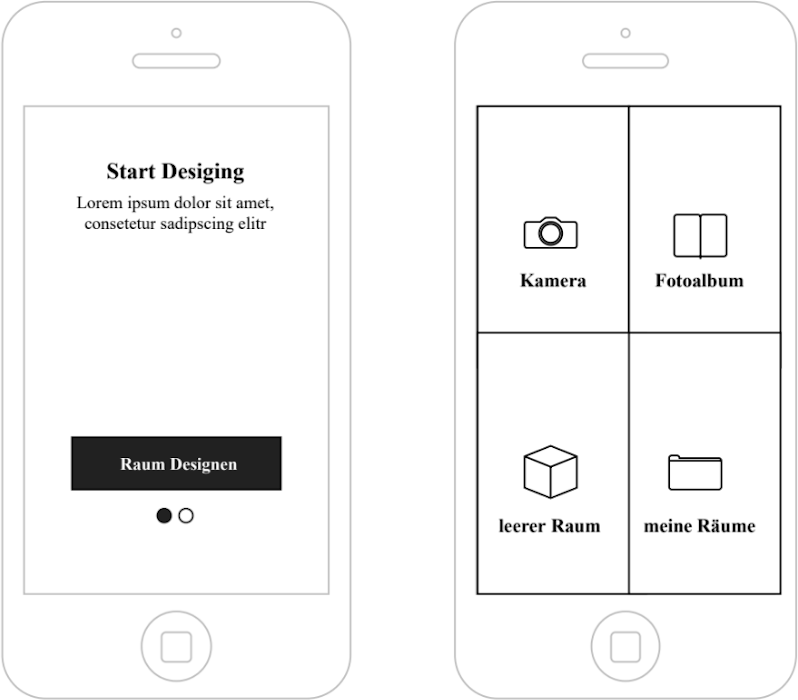
\includegraphics[height=200px]{./img/m2_lofi_sophia_12.png}
\caption{\label{fig:lofi_sophia_12}Prototype Sophia: Screens 1 -- 2}
\end{figure}

Am zweite Start Screen, den man durch einmal nach links wischen sehen
kann, steht „Discover Ideas“, auch eine kurze Beschreibung und einen
Button mit „Katalog durchstöbern"`. Hier würde ich als Hintergrundbild
ein Foto von einem schlichten Möbelstück oder ähnliches platzieren.
Betätigt man den Button kommt man zu einem Screen
(\textbf{Abb. \ref{fig:lofi_sophia_34}}) mit Fotos und Ideen.  Oben ist eine Slideshow
mit fertig gestalteten

\begin{figure}[htbp]
\centering
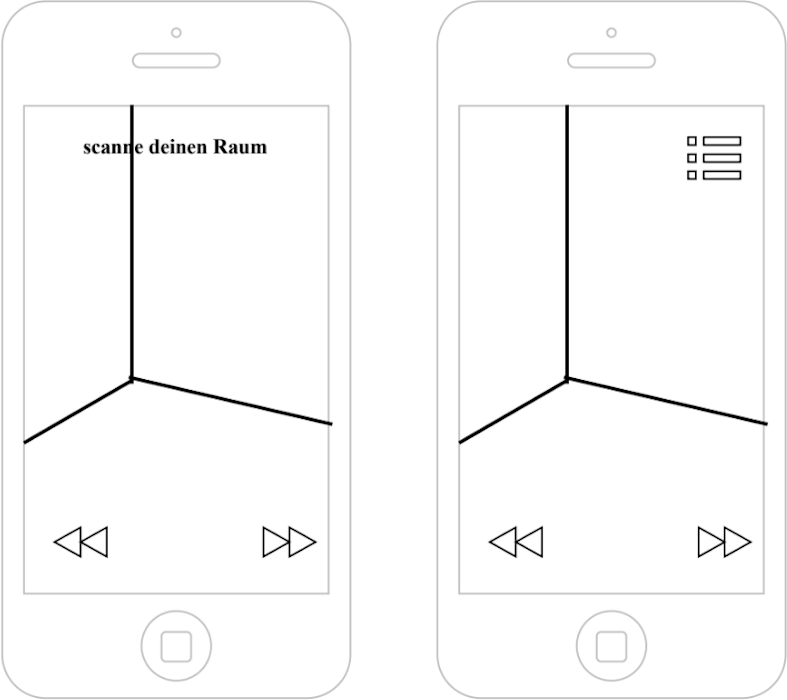
\includegraphics[height=200px]{./img/m2_lofi_sophia_34.png}
\caption{\label{fig:lofi_sophia_34}Prototype Sophia: Screens 3 -- 4}
\end{figure}

Wohnräumen, die zur Inspiration dienen sollen. Man kann sie durch
wischen steuern oder anklicken und durch eine Fotogalerie navigieren
(\textbf{Abb. \ref{fig:lofi_sophia_56}}).  Unter der Slideshow steht „Wohnideen“ und
darunter findet man verschieden Kategorien, die durch Icons und Namen
dargestellt werden und verschiedene Möbelstücke anzeigen lassen. Unter
„Meine Möbel“ kann man selbst Möbel einscannen und in der App
abspeichern.

\begin{figure}[htbp]
\centering
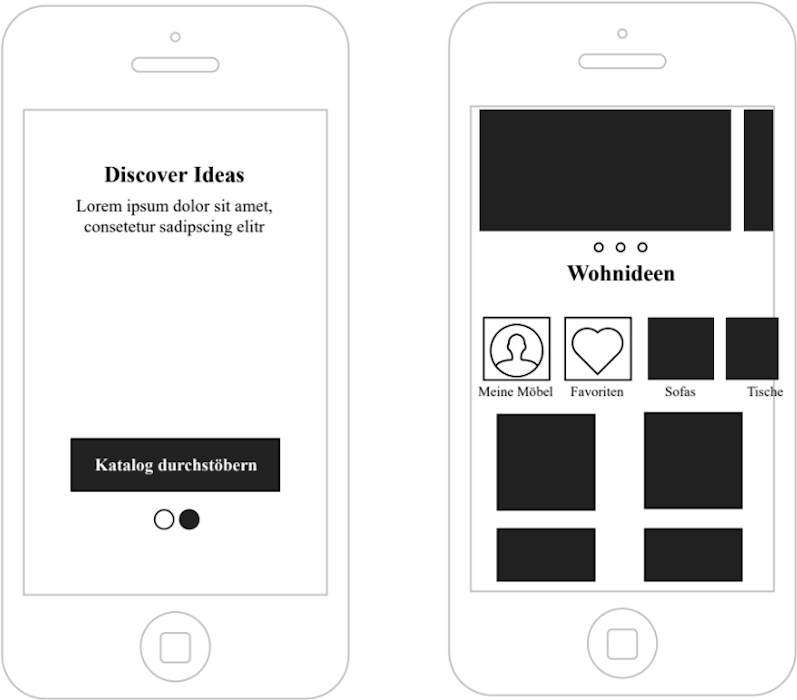
\includegraphics[height=200px]{./img/m2_lofi_sophia_56.png}
\caption{\label{fig:lofi_sophia_56}Prototype Sophia: Screens 5 -- 6}
\end{figure}

\subsection{Prototyp von Asım}
\label{sec:orga3e5932}
\emph{Autor: Asım OĞUZ}

\textbf{Abb. \ref{fig:lofi_asim_1}} zeigt eine simple Startseite, auf der man gleich den ersten
Schritt sieht den man machen muss. Und zwar
einen Raum zum Gestalten auswählen.

\begin{figure}[htbp]
\centering
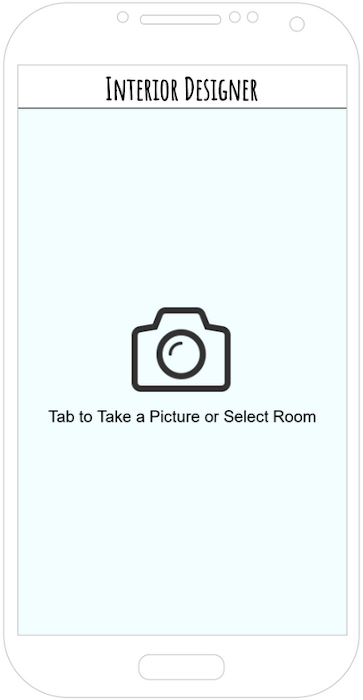
\includegraphics[height=200px]{./img/m2_lofi_asim_1.png}
\caption{\label{fig:lofi_asim_1}Prototype Asım: Screen 1}
\end{figure}

Auf \textbf{Abb. \ref{fig:lofi_asim_2}} gibt es zwei Möglichkeiten einen Raum auszuwählen:

\begin{enumerate}
\item Raum fotografieren

Bei diesem Schritt wird die Kamera geöffnet und
der User kann den gewünschten Raum
fotografieren und das Bild importieren.

\item Einen Raum aus den Vorhandenen Designs auswählen
\end{enumerate}

\begin{figure}[htbp]
\centering
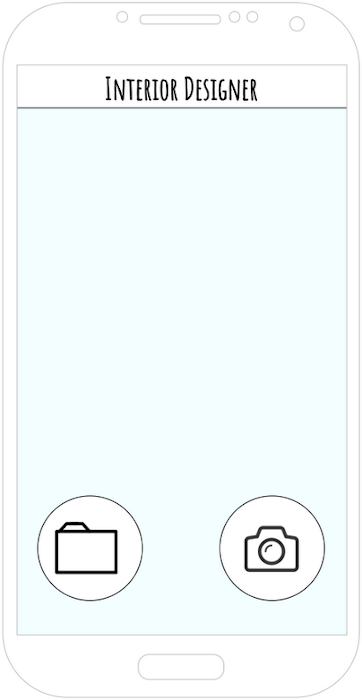
\includegraphics[height=200px]{./img/m2_lofi_asim_2.png}
\caption{\label{fig:lofi_asim_2}Prototype Asım: Screen 2}
\end{figure}

\textbf{Abb. \ref{fig:lofi_asim_3}}: Falls man einen Raum aus den Vorhandenen
Designs auswählen möchte werden die als Liste die
man durchscrollen kann angezeigt. Durch einen Tab
kann man ein Design auswählen.

\begin{figure}[htbp]
\centering
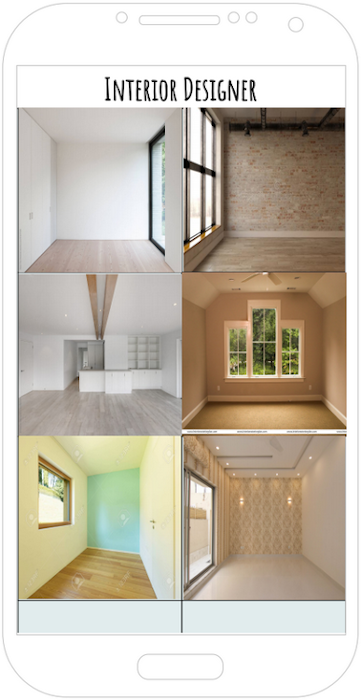
\includegraphics[height=200px]{./img/m2_lofi_asim_3.png}
\caption{\label{fig:lofi_asim_3}Prototype Asım: Screen 3}
\end{figure}

Nach dem ein Raum ausgewählt wurde besteht auf \textbf{Abb. \ref{fig:lofi_asim_4}} die
Möglichkeit Möbel zu importieren. Dies geschieht in
dem man auf das "`+"' Button klickt.

\begin{figure}[htbp]
\centering
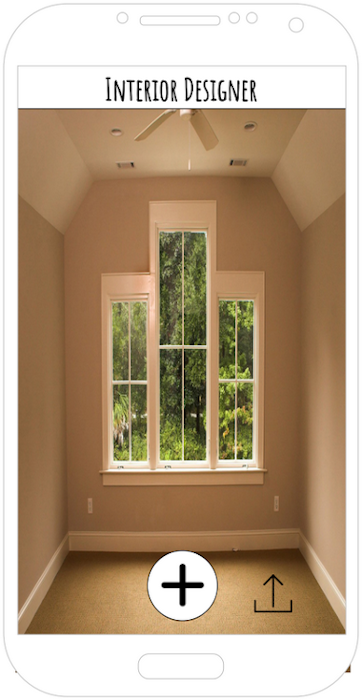
\includegraphics[height=200px]{./img/m2_lofi_asim_4.png}
\caption{\label{fig:lofi_asim_4}Prototype Asım: Screen 4}
\end{figure}

In \textbf{Abb. \ref{fig:lofi_asim_5}} kann man durch das Berühren eines
Möbelstückes dieses in den Raum importieren.

\begin{figure}[htbp]
\centering
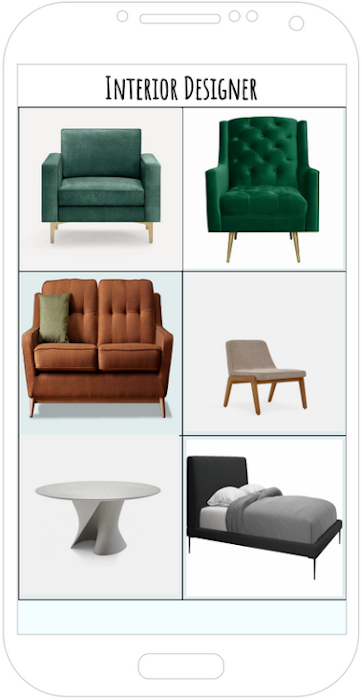
\includegraphics[height=200px]{./img/m2_lofi_asim_5.png}
\caption{\label{fig:lofi_asim_5}Prototype Asım: Screen 5}
\end{figure}

\textbf{Abb. \ref{fig:lofi_asim_6}}: Der Schritt zum Möbel importieren wird mehrmals ausgeführt bis man
alle gewünschten Möbel sieht.  Die Importieren Möbel können durch
zeihen durch den Raum bewegt und an die gewünschte Position gebracht
werden.  Sobald der Raum nach Wunsch gestaltet wurde kann man ihn mit
dem Export Button in die Galerie abspeichern.

\begin{figure}[htbp]
\centering
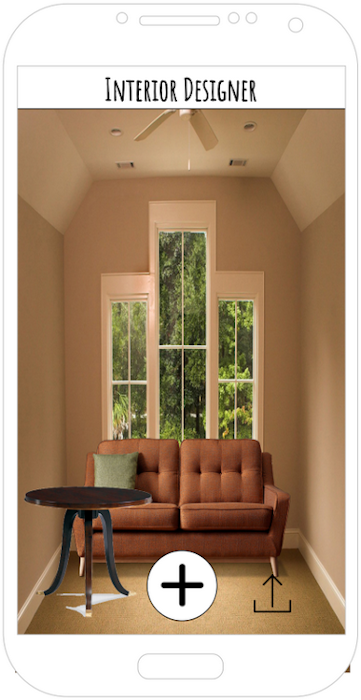
\includegraphics[height=200px]{./img/m2_lofi_asim_6.png}
\caption{\label{fig:lofi_asim_6}Prototype Asım: Screen 6}
\end{figure}

\subsection{Prototyp von Dominik}
\label{sec:org420f740}
\emph{Autor: Dominik Pegler}

Mein Ziel war es, eine grobe Skizze einer Interior-Designer-App
anzufertigen, die vor allem auf die Punkte aus der Mindmap abzielt,
die eine einfache Bedienung und ein reduziertes UI forcieren.

Die Abb. \textbf{\ref{fig:lofi_dominik_1}} stellt den Erstkontakt der User mit der
App dar. Die App fragt die User, was sie denn jetzt machen möchten und
gibt ihnen dabei zwei Optionen: (1) eine Seite mit früheren Projekten
aufzurufen oder (2) ein neues Projekt zu beginnen ("`start
scanning"'). Man könnte hier bereits einen Button für Einstellungen
integrieren, in diesem ersten Designvorschlag fehlt dieser jedoch
noch.

\begin{figure}[htbp]
\centering
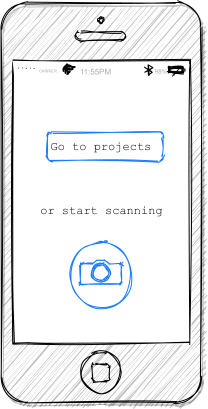
\includegraphics[height=200px]{./img/m2_lofi_dominik_1.png}
\caption{\label{fig:lofi_dominik_1}Prototype Dominik: Screen 1}
\end{figure}

Gehen wir davon aus, dass ein User oder eine Userin den Button mit der
Kamera angetippt hat, so finden wir uns in Abb. \textbf{\ref{fig:lofi_dominik_23}}
wieder -- im Scanprozess. Um die App mit möglichst großer Menge an
Daten zu versorgen, werden die User gebeten, sich im Raum
herumzudrehen. Die App gibt vor, welche Bereiche im Raum noch mehr
Scandurchgänge benötigen, um ein präzise Berechnung der Raummaße
möglich zu machen. Eine Statusleiste zeigt den Fortschritt im
Scanprozess an. Die User können den Scanprozess jederzeit mit
Berührung des X-Buttons abbrechen. Ansonsten ist dieser beendet, wenn
die App ausreichend Informationen zur Berechnung des Raums hat,
visualisiert durch das Symbol mit dem Häkchen und der knappen Message
"`finished!"'.

\begin{figure}[htbp]
\centering
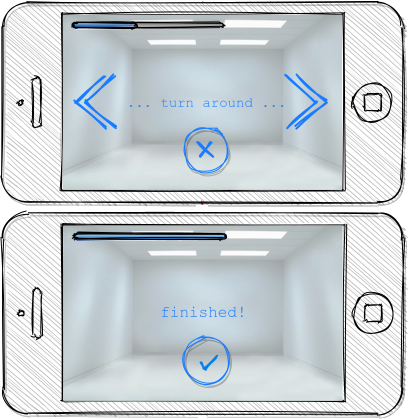
\includegraphics[height=200px]{./img/m2_lofi_dominik_23.png}
\caption{\label{fig:lofi_dominik_23}Prototype Dominik: Screens 2 -- 3}
\end{figure}

Nach dem erfolgreichen Scanprozess teilt die App den Usern mit, zu
welchem Ergebnis sie gekommen ist (Abb. \textbf{\ref{fig:lofi_dominik_45}}). Sie
möchte vom User nur noch kurz wissen, ob sie ihre Arbeit gut gemacht
hat und die Maße des Raumes stimmen. Ist das der Fall, betätigt der
User oder die Userin den Button mit dem Häkchen und gelangt ins Menü
zur Auswahl der Gegenstände, die man im Raum platzieren kann. Man kann
hier über ein Suchfeld nach Objekten suchen oder durch eine Liste an
Objekten (selbst erstellte wie auch Beispiel-Objekte) scrollen.

\begin{figure}[htbp]
\centering
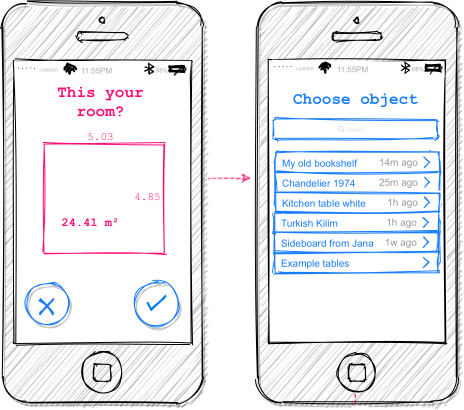
\includegraphics[height=200px]{./img/m2_lofi_dominik_45.png}
\caption{\label{fig:lofi_dominik_45}Prototype Dominik: Screens 4 -- 5}
\end{figure}

Hat man sich für ein Objekt entschieden (Abb. \textbf{\ref{fig:lofi_dominik_67}}),
wird dieses Objekt am Bildschirm angezeigt. Man kann dieses dann über
die Pfeil-Buttons drehen und damit von verschiedenen Seiten
betrachten. Tippt man erneut auf das Objekt, wird es dem Raum
hinzugefügt. Dabei ermittelt die App eine freie Stelle und platziert
das Objekt im Raum. Die User können das Objekt durch Antippen und
Ziehen im Raum bewegen. Weitere Prototypen-Skizzen sollen an diese
erste Studie anknüpfen und die gezeigten Funktionalitäten mit mehr
Detailreichtum demonstrieren.

\begin{figure}[htbp]
\centering
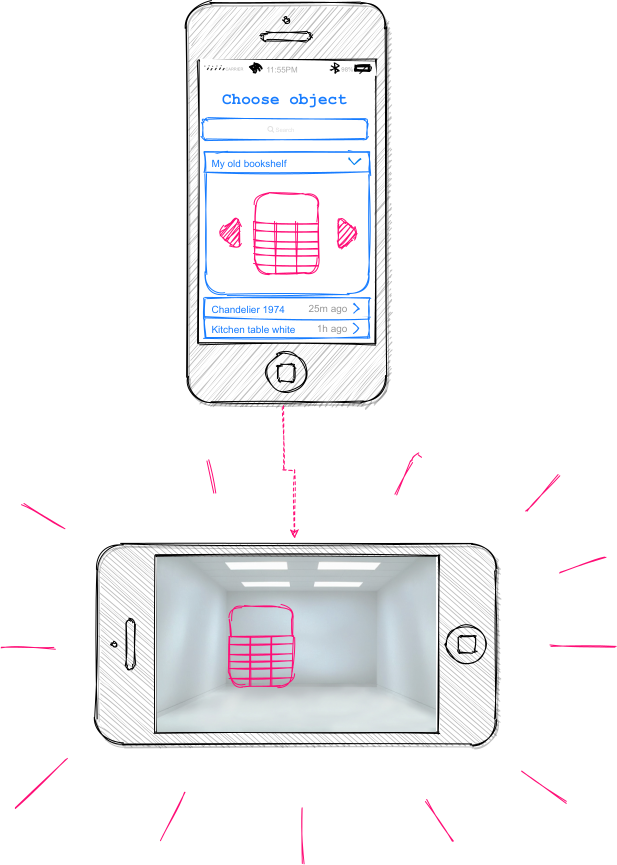
\includegraphics[height=422px]{./img/m2_lofi_dominik_67.png}
\caption{\label{fig:lofi_dominik_67}Prototype Dominik: Screens 6 -- 7}
\end{figure}
\section{Evaluierung der Prototypen}
\label{sec:org6108321}
\subsection{Prototyp von Sophia}
\label{sec:org1934dfa}

\subsubsection{\textbf{Feedback von Person A} (\emph{Autor: Asım OĞUZ})}
\label{sec:org5ebaf88}

Die erste Seite dieses Prototypen sieht zu leer aus diesem würde ein
Hintergrundbild weiterhelfen. Der zweite Screen ist simpel und
verständlich alle Funktionen sind ersichtlich, diese Seite ist gut
designt, jedoch könnte man vielleicht bei der Kamera dazu schreiben,
dass man scannt und nicht fotografiert. Auf der Scan Seite ist unklar
wie man den Scan abschließt bzw. beendet. Es ist unklar was man nach
dem Scannen machen muss. Wie fügt man Möbel hinzu? Wie speichert man
ab? Diese fragen bleiben unbeantwortet. Die letzte Seite, die mit
Wohnideen, ist eher wie eine Desktop Webseite aufgebaut, daher sind
die Bilder zu klein. Hier würde es helfen die Abstände zwischen den
Bilder zu verkleinern, dadurch würde man Platz gewinnen, welches man
für die Vergrößerung der Bilder benutzen kann.

\subsubsection{\textbf{Feedback von Person B} (\emph{Autorin: Sophia PUM})}
\label{sec:org93ca253}
Dieser Prototyp ist auch sehr minimal gestaltet und obwohl ein klare Design gut passt könnten, vor allem die ersten beiden Home-Screens, etwas lebhafter gemacht werden, z.B. durch Bilder oder Farben. Das Menü beim „Raum Designen“ wird durch die vier Felder gut dargestellt. Durch die Wörter und Icons ist klar welche Funktion dahinter steckt. Allerdings ist es nicht ganz nachvollziehbar was genau jetzt passiert wenn man z.B. auf „Kamera“ drückt. Beim Raum bearbeiten ist das Icon um Möbel einzufügen nicht sehr optimal, bzw. fehlt dafür eine Beschreibung. Der Katalog ist schön und sehr übersichtlich gelöst.  Eventuell sind es zu viele Fotos auf einmal, was sich vielleicht dem sonstigen minimalistischen Design widerspricht.
\subsubsection{\textbf{Feedback von Person C} (\emph{Autor: Dominik Pegler})}
\label{sec:org34b2364}

Die interviewte Person zeigte sich zunächst über den Satz "`Start
Desiging"' am Startbildschirm irritiert, fand sich dann aber relativ
schnell im Design zurecht.

Am zweiten Bildschirm war die Bedeutung der Icons nicht ganz
klar. Inbesondere fragte die Person nach der Bedeutung von "`Kamera"'
und "`Fotoalbum"': "`Warum sollte ich jetzt auf Fotoalbum klicken? Mir
ist das nicht klar."' Es wäre vielleicht gut, eine kurze Beschreibung
anzufügen oder zumindest einen sprechendere Untertitel, welche
Funktion mit diesen Buttons ausgelöst werden.

Zum Gesamteindruck meinte der Testuser, dass das UI insgesamt sehr
nüchtern sei und er es für eine App dieser Art gerne etwas bunter und
kreativer hätte. Auf der anderen Seite sei es aber auch wiederum cool,
dass das Design so aufgeräumt wirkt.

Während der Beurteilung dieses Prototypen kamen dem Testuser auch
Ideen für Erweiterungen: So könnte man beispielsweise auch Pflanzen
integrieren, und eine Art "`Randomfunktion"', bei der ein Zufallsartikel
(der dann bei einem Webshop gekauft werden kann) automatisch im Raum
platziert wird, für Überraschung sorgen könnte.

\subsection{Prototyp von Asım}
\label{sec:org15a76ed}

\subsubsection{\textbf{Feedback von Person A} (\emph{Autor: Asım OĞUZ})}
\label{sec:org3b182da}

Das erste was an diesem Prototypen auffällt ist die Navbar mit dem
Namen “Interior Designer”, diese ist auf allen Seiten der App zu
sehen, jedoch verschönert dies das Design nicht und sollte weggelassen
bzw. überarbeitet werden. Weiters ist die Farbe für die Hintergründe
auf den ersten zwei Seiten nicht gut aussehend und sollte durch ein
passendes Foto ersetzt werden. Die zweite Seite ist zu simpel gehalten
und ein bisschen unverständlich, das Icon, welches zum Auswählen aus
den Vorhandenen Räumen gedacht ist, lässt vermuten, dass man in die
eigene Galerie kommt. Hier sollte das Icon geändert und eine
Beschriftung hinzugefügt werden. Die Seiten zum auswählen der Räume
und Möbel sind durch die großen Bilder übersichtlich, jedoch würde
diesen Seiten eine Kategorisierung bzw. eine Suchfunktion
weiterhelfen.

\subsubsection{\textbf{Feedback von Person B} (\emph{Autorin: Sophia PUM})}
\label{sec:orgb9a7811}

Oberfläche ist einfach und minimal gestaltet. Obwohl es wenig Text gibt, ist in jedem Screen im Großen und Ganzen klar welche Funktionen es gibt, denn das Design simpel ist, den Gewohnheiten der NutzerInnen und Nutzer entspricht und keine verspielten Details beinhaltet.  Die Startseite und der zweite Screen könnten durch Fotos oder ähnliches etwas ansprechender gestaltet werden. Das Icon für „Select a Room“ stellt die Funktion auch nicht ganz optimal dar. Auch wenn man dann den Raum einrichtet, wären ein paar kurze Stichworte zur Beschreibung sinnvoll. Der Schriftzug „INTERIOR DESIGNER“ der auf jedem Screen abgebildet ist, sollte vielleicht überarbeitet werden, er wirkt etwas dominant und es wäre besser in z.B. durch ein Icon/Logo zu ersetzen.
\subsubsection{\textbf{Feedback von Person C} (\emph{Autor: Dominik Pegler})}
\label{sec:orga6281de}

Der Testuser fand die Schriftart zum Schriftzug "`INTERIOR DESIGNER"'
nicht so passend. Sie wirke wackelig und vermittle Unsicherheit. Dabei
solle die App einem ja Sicherheit bei einer Entscheidungsfindung
geben.

Zum Prozess der Auswahl von Raum und Möbelstück meinte der Testuser,
dass es nicht ganz klar sei, wie die Abmessungen zustande kämen, wie
der Platz berechnet werde, ob die Proportionen stimmen würden und wie
viele Restplatz übrig bliebe, nachdem man das Möbelstück platziert
hat. Hier würde sich der Testuser ein paar Maßangaben wünschen.

Zum letzten Screen meinte der Testuser, dass nicht klar sei, wofür die
beiden Buttons (Das Plus-Symbol und das Upload-Symbol) stehen und
worin sie sich unterscheiden.

Der Gesamteindruck wurde als nüchtern bewertet. Es fehle etwas, das
einen einlädt kreativ tätig zu werden und den Spaß am Gestalten
vermittelt. Als konkretes Beispiel wurden dabei Animationen (Vorhang
auf) während der Ladezeiten genannt.

\subsection{Prototyp von Dominik}
\label{sec:org0f5a328}

\subsubsection{\textbf{Feedback von Person A} (\emph{Autor: Asım OĞUZ})}
\label{sec:org1541510}

Die erste Seite dieses Prototypen sieht zu leer aus diesem würde ein
Hintergrundbild weiterhelfen. In der Seite, die zum Scannen des Raumes
dient, gibt es einige Aspekte die unklar sind. Wird der Scan
automatisch beendet? Wenn nicht fehlt ein Button um dies zu
machen. Was macht das Button “X”? Bricht dies den ganzen Vorgang ab
oder beginnt man von Anfang an zu scannen? Dem würde eine Beschriftung
weiterhelfen. Und falls dieser Button den Vorgang abbricht würde ein
“Try Again” Button gut passen. Die Seite zum auswählen von Möbeln ist
sehr übersichtlich und verständlich und daher passend. Auf der letzen
Seite sind gar keine Buttons. Kann man da keine weiteren Möbel mehr
hinzufügen? Wie exportiert man den Raum? Diese Fragen sind unklar.

\subsubsection{\textbf{Feedback von Person B} (\emph{Autorin: Sophia PUM})}
\label{sec:org428ce8f}
Auch hier ist die Nutzeroberfläche sehr übersichtlich und klar gestaltet. Gut an diesem Entwurf ist, dass es trotz dem minimalen Stil kurze Beschreibungen gibt, die die Bedienung für die Nutzerinnen und Nutzer einfacher machen. Die Texte sind kurz und knapp, das ist angenehm für den Benutzer, denn man kann sie schnell lesen und sie beinhalten nichts Überflüssiges. Der Screen „Choose Object“ ist mit dem Drop-Down-Menü auch sehr einfach zu bedienen, denn diese Art von Menü ist jedem Internet-Nutzer bekannt. Hier wäre vielleicht eine Möglichkeit die Möbel zu sortieren oder zu filtern sinnvoll.

\subsubsection{\textbf{Feedback von Person C} (\emph{Autor: Dominik Pegler})}
\label{sec:org91059cb}

Der Testuser war nicht ganz einverstanden mit der Formulierung des
Satzes "`This your room?"' Er würde das anders formulieren. Außerdem sei
nicht klar, was die Phrase "`start scanning"' am Startbildschirm
bedeute. Falls das ein neues Projekt sei, sollte es auch so benannt
werden, sagte der Tester.

Des Weiteren sollte der Button für das "`Neue"' oben sein und der Button
für das "`Alte"', also die alten Projekte, unten. Das sei intuitiver und
kenne der Testuser aus anderen Apps.

Die Rückmeldungen der App mit "`turn around"' und "`finished"' mit dem
Häckchen fand der Tester wiederum gut. Nicht so klar war die Bedeutung
des "`X"' und des Häkchens am Bildschirm mit dem Satz "`this your
room?"'. Der Tester konnte sich keine Vorstellung machen, was nun
passieren würde, wenn er das "`X"' antippt. Er fragte: "`Muss ich dann
selber abmessen gehen?"'

Der berichtete Gesamteindruck war, dass das UI frisch aussieht
(zumindest von der Farbgebung her) und der Designvorschlag etwas
konkreter ist, was die Raum-Abmessungen und Auswahl von
Einrichtungsgegenständen betrifft.

\section{Anpassung der Prototypen}
\label{sec:orgffb7cb0}
\emph{Autor*innen: Dominik PEGLER, Sophia PUM, Asım OĞUZ}
\subsection{Prototyp von Sophia}
\label{sec:org3833639}
\begin{itemize}
\item Scanseite überarbeiten
\item Screen 6 für mobile Geräte anpassen (simpler)
\item Funktion implementieren, um Möbel hinzuzufügen (Button, Menü usw.)
\item Kurze Hinweistexte unter die Buttons, damit Funktion klarer
\end{itemize}

\subsection{Prototyp von Asım}
\label{sec:orga0e1332}
\begin{itemize}
\item Mehr Beschreibung am 2. Screen
\item Möbel in Kategorien gliedern
\item Suchmöglichkeit integrieren
\item Navigationsleiste sollte je nach Screen unterschiedlich
\item Infoliste für jeden Screen, um sichtbar zu machen, wo man sich gerade befindet
\item Kurze Beschreibung zu den einzelnen Möbeln und Kategorien
\item Anordnung der Bilder überbearbeiten
\item Schriftzug „INTERIOR DESIGNER“ überarbeiten (eventuell Logo)
\end{itemize}
\subsection{Prototyp von Dominik}
\label{sec:orgd706e48}
\begin{itemize}
\item Während des Scanvorgangs mehr Informationen
\begin{itemize}
\item Abbruch-Button farblich besser kennzeichen
\item Statusleiste besser hervorheben
\end{itemize}
\item Button implementieren für zusätzliche Möbel in bereits gestaltetem Raum
\item Button implementieren für Export des fertigen Raumes
\item Startscreen ansprechender gestalten
\begin{itemize}
\item Hintergurndbild
\item Anordnung der Buttons umkehren
\end{itemize}
\item Funktion hinzufügen um gespeicherte Möbel zu
\begin{itemize}
\item kategorisieren
\item sortieren
\item filtern
\end{itemize}
\end{itemize}

\subsection{Zusätzliche zielgruppenspezifische Anpassungen für alle 3 Prototypen}
\label{sec:orgbed85f4}

\begin{itemize}
\item Farbenfroheres Design implementieren
\item Hintergrundbilder und Wallpapers implementieren
\item Default-Schriftarten festlegen
\item Farbpalette festlegen
\end{itemize}
\end{document}
